% !TeX root = ../main.tex
\chapter{人机协同柔性物体操作综合实验验证}
\label{chap:dual_arbitration_industrial_contact}
\label{chap:ch5_integrated_validation}

第三章围绕柔性接触操作中的执行层控制问题，建立了基于合作博弈的力位协同控制器，使机器人能够在位置轨迹精度和接触力安全之间形成可调折中。第四章进一步面向人在环操作过程，给出了参考层动态仲裁方法，将操作者输入解释为安全参考修正，并通过接触安全投影削弱可能引起法向过压的危险输入。前两章分别解决执行层力位协调和参考层人机仲裁问题，但真实柔性物体操作通常同时包含环境刚度变化、操作者在线修正、接触力边界和几何边界条件。单一模块验证只能说明局部性质，综合实验需要进一步考察两类模块在同一机器人系统中的配合关系。

本章面向人机协同柔性物体操作开展综合实验验证，重点放在统一系统、统一工况、统一方法接口和统一指标下的组合效果分析。合作博弈反馈律和动态仲裁规则沿用第三章、第四章的设计，本章主要组织控制器、仲裁器和完整组合方法的对比。实验对象覆盖两类典型边界条件：一类为无远心运动约束的柔性表面接触操作，用于检验方法在一般柔性工件上的适用性；另一类为带远心运动约束的长工具柔性接触操作，用于检验方法在固定点轴线边界下的可执行性。通过统一平台、统一数据记录、统一方法建模和统一评价指标，本章为后续仿真和实物实验结果分析建立共同基础。

\section{综合验证目标}
\label{sec:ch5_validation_goal}

综合验证的核心任务是考察第三章执行层控制器和第四章参考层仲裁器在同一闭环系统中的兼容性。执行层控制器根据接触力安全裕度和环境刚度估计调整力位优先级，主要影响机器人对给定参考轨迹的跟踪方式；参考层仲裁器根据操作者输入强度、持续性、方向一致性和接触安全状态调整人机仲裁权重，主要影响最终期望轨迹的生成方式。两类模块作用层级不同，评价时也需要分别观察力安全、轨迹质量、人类修正保留程度和系统实时性。

本章综合验证围绕四个问题展开。第一，执行层力位协同控制器接入人机参考后，是否仍能在变刚度柔性接触中控制接触力越界时间，并保持合理轨迹误差。第二，参考层动态仲裁器接入执行层控制器后，是否能够保留安全切向修正，同时削弱危险法向压入。第三，两层模块组合后，仲裁参数、控制输入和计算时间是否满足实时机器人实验的可执行要求。第四，在无远心运动约束和带远心运动约束两类任务中，完整组合方法是否表现出一致、可解释的综合趋势。

上述验证问题在实验中分别落实为四类可观测现象。执行层力位协调能力主要通过变刚度区域内的接触力响应体现：若动态力位优先级有效，则高刚度或力安全裕度降低时的力越界时间应减少，轨迹误差仍应保持在任务允许范围内，相应指标包括接触力均方根误差、力越界时间和轨迹均方根误差。参考层人机仲裁能力主要通过操作者输入的处理结果体现：安全切向修正应进入最终期望轨迹，可能导致过压的法向压入应被削弱，相应指标包括人类修正接受率、危险输入抑制率和接触力峰值。组合闭环可执行性主要通过在线运行状态体现，两类仲裁参数应连续变化，控制输入不应出现不必要突跳，单周期计算时间应满足机器人实时执行要求。跨边界条件适用性则通过两类实验任务共同验证：无远心运动约束的柔性表面接触实验重点观察力安全、轨迹质量和人类切向修正保留，带远心运动约束的长工具实验在上述指标之外进一步观察固定点轴线几何误差。

本章结论应围绕综合表现展开。在某些单项指标上，固定参数方法或单层方法可能具有局部优势，例如强力优先策略可能得到较低的接触力均方根误差，强位置优先策略可能得到较小的切向轨迹偏差。综合验证关注的是多项指标之间的协调关系：接触力越界时间能否下降，人类安全修正能否保留，危险输入能否抑制，控制周期能否满足在线执行。后续实验分析将以这一目标为边界，避免把单项数值优势扩大为全局结论。

\section{统一实验系统}
\label{sec:ch5_system}

综合验证需要保证不同方法在相同平台、相同任务、相同输入序列和相同安全条件下比较。本章采用统一实验系统描述仿真与实物实验，使后续结果能够对应到同一套变量和指标。系统由操作者输入、参考层动态仲裁、执行层力位协同控制、机器人接触执行、柔性环境反馈和安全监督六个部分组成。操作者输入首先被解释为候选人侧参考，经过第四章方法生成安全参考和人机仲裁权重；执行层随后调用第三章控制器，根据最终期望轨迹、期望接触力和实时力反馈计算机器人控制输入；安全监督层对力阈值、速度限幅、工作空间边界和急停条件进行统一约束。

统一系统的信号流可概括为
\begin{equation}
  \{x_r,s_h,y_f,\hat K_e\}
  \longrightarrow
  \{x_h^{\mathrm{safe}},\alpha_{\mathrm{HR}},x_d\}
  \longrightarrow
  \{\alpha_{\mathrm{FP}},u\}
  \longrightarrow
  \{x,y_f,e_{\mathrm{gc}}\},
  \label{eq:ch5_system_flow}
\end{equation}
其中 $x_r$ 为机器人自主参考，$s_h$ 为操作者输入，$y_f$ 为受控法向接触力，$\hat K_e$ 为环境刚度估计，$x_h^{\mathrm{safe}}$ 为经过安全投影的人侧参考，$\alpha_{\mathrm{HR}}$ 为人机仲裁权重，$x_d$ 为最终期望轨迹，$\alpha_{\mathrm{FP}}$ 为执行层力位优先级，$u$ 为任务空间控制输入，$x$ 为实际末端接触点位置，$e_{\mathrm{gc}}$ 为长工具任务中的固定点轴线几何误差。式\eqref{eq:ch5_system_flow}只用于说明实验系统的数据流和模块接口，具体控制律和仲裁规则沿用第三章和第四章。

仿真实验和实物实验使用相同信号定义和评价指标。实物平台以 Franka 机械臂或等效七自由度机械臂为执行主体，记录关节状态、末端位姿、控制输入和计算周期。操作者输入由主端设备、手柄或预设输入序列给出，用于形成安全切向修正、持续目标重定向、短时扰动和危险法向压入。力反馈可来自末端六维力传感器或机器人外力估计，实验开始前需要完成零偏校准，并将测量结果转换到任务坐标系下的受控法向力。无远心运动约束任务主要使用圆头探针或短杆接触海绵、硅胶块、泡棉等柔性材料，通过软区、硬区和局部缺陷区域触发力位调节和人类修正需求。带远心运动约束任务使用长工具通过固定孔、套管或虚拟远心运动点接触柔性对象，固定点轴线几何误差只作为该类长工具任务的附加评价边界，不改变全文以人机协同柔性物体操作为主的研究定位。所有实验均由统一安全监督层限制接触力硬阈值、末端速度、工作空间和急停条件，硬安全事件单独记录，不作为算法性能改善的直接证据。

为保证仿真和实物实验具有可比性，所有方法均记录同一组基础数据。记录量包括时间戳、关节位置和速度、末端位姿、末端速度、机器人自主参考、人侧候选参考、安全人侧参考、最终期望轨迹、接触力、期望接触力、力位优先级、人机仲裁权重、力安全裕度、环境刚度估计、操作者输入和单周期计算时间。对于长工具任务，还需记录工具轴线参数和固定点轴线几何误差。后续图表均由这些实验记录计算得到，正文只呈现实验系统、指标定义和结果现象。

数据处理采用统一规则。每组方法在相同任务条件下完成重复试次，统计前先检查力传感器零偏、通信状态、机器人急停、工具有效接触和任务指令完成情况。若出现传感器明显掉线、通信中断、硬安全急停或工具未形成有效接触等工程异常，该试次可单独标记并说明原因。正常范围内的力峰值、轨迹误差和人类输入波动应保留在统计中。每组实物实验建议至少重复三次，条件允许时重复五次；表格给出均值和标准差，曲线图展示典型试次，箱线图展示离散程度。

\section{综合方法建模}
\label{sec:ch5_integrated_model}

综合实验的方法建模用于明确两类仲裁在同一闭环中的位置。参考层人机仲裁负责把操作者输入转化为安全期望轨迹，执行层力位仲裁负责在给定期望轨迹和期望接触力条件下调节反馈控制优先级。两层变量分别记为 $\alpha_{\mathrm{HR}}(t)$ 和 $\alpha_{\mathrm{FP}}(t)$：前者描述人侧参考对最终期望轨迹的影响程度，后者描述执行控制中位置目标和力目标的相对权重。这样的分层建模使第五章能够在统一实验中同时观察人类修正保留、危险输入抑制、接触力边界保持和轨迹执行质量。

\subsection{参考层轨迹仲裁模型}
\label{subsec:ch5_reference_arbitration_model}

设操作者输入 $s_h(t)$ 经过主从比例映射后形成候选人侧参考修正 $\Delta x_h(t)$，机器人自主参考为 $x_r(t)$，则候选人侧参考写为
\begin{equation}
  x_h(t)=x_r(t)+K_h\Delta x_h(t),
  \label{eq:ch5_human_candidate_model}
\end{equation}
其中 $K_h$ 为主从比例矩阵。式\eqref{eq:ch5_human_candidate_model}只表示参考层的监督修正，候选参考还需经过意图判断和接触安全筛选后才能进入执行层。

参考层仲裁依据人类输入强度、持续时间、方向一致性和空间风险等特征生成目标权重。记
\begin{equation}
  \eta_h(t)=
  \begin{bmatrix}
    I_h(t) & T_h(t) & C_h(t) & R_s(t)
  \end{bmatrix}^{\mathrm T},
  \label{eq:ch5_human_feature_vector}
\end{equation}
其中 $I_h$ 表示归一化干预强度，$T_h$ 表示持续时间特征，$C_h$ 表示人侧修正方向与自主参考方向的一致性，$R_s$ 表示由工作空间边界、几何误差裕度或任务区域给出的风险特征。目标人机仲裁权重为
\begin{equation}
  \alpha_{\mathrm{HR},r}(t)=
  \mathcal A_{\mathrm{HR}}\bigl(\eta_h(t),\rho_F(t),e_{\mathrm{gc}}(t)\bigr),
  \label{eq:ch5_alpha_hr_map}
\end{equation}
其中 $\mathcal A_{\mathrm{HR}}(\cdot)$ 沿用第四章的动态仲裁映射，$\rho_F$ 为接触力安全裕度，$e_{\mathrm{gc}}$ 为长工具任务中的固定点轴线几何误差。为避免人侧权重突变，实验中采用一阶滤波得到实际仲裁权重：
\begin{equation}
  \dot{\alpha}_{\mathrm{HR}}(t)=
  \lambda_{\mathrm{HR}}
  \bigl(\alpha_{\mathrm{HR},r}(t)-\alpha_{\mathrm{HR}}(t)\bigr),
  \quad
  0\le \alpha_{\mathrm{HR}}(t)\le 1,
  \label{eq:ch5_alpha_hr_filter_model}
\end{equation}
其中 $\lambda_{\mathrm{HR}}>0$ 为参考层响应速度。该参数越大，系统越快响应操作者修正；该参数越小，最终期望轨迹越平滑。

柔性接触任务中，人侧候选参考需要同时满足接触力边界。设 $n_c(t)$ 为接触法向，$\hat K_e(t)$ 为环境等效刚度估计，则候选点 $\bar x$ 对应的局部接触力预测为
\begin{equation}
  \hat F(\bar x;t)=
  y_f(t)+\hat K_e(t)n_c^{\mathrm T}(t)\bigl(\bar x-x(t)\bigr).
  \label{eq:ch5_force_prediction_model}
\end{equation}
由力边界、工作空间和可选几何边界构造安全参考集合
\begin{equation}
  \mathcal X_s(t)=
  \left\{
  \bar x\in\mathcal X_{\mathrm{ws}}
  \ \middle|\
  F_{\min}+\Delta_F\le \hat F(\bar x;t)\le F_{\max}-\Delta_F,\
  e_{\mathrm{gc}}(\bar x)\le e_{\mathrm{gc}}^{\max}
  \right\},
  \label{eq:ch5_safe_reference_set}
\end{equation}
其中 $\mathcal X_{\mathrm{ws}}$ 为实验工作空间，$\Delta_F>0$ 为力安全余量。无远心运动约束任务可令 $e_{\mathrm{gc}}(\bar x)=0$。人侧安全参考定义为
\begin{equation}
  x_h^{\mathrm{safe}}(t)=
  \arg\min_{\bar x\in\mathcal X_s(t)}
  \left\|\bar x-x_h(t)\right\|^2.
  \label{eq:ch5_safe_projection_model}
\end{equation}
该投影保留离候选参考最近的安全点，因此安全切向修正能够尽量保留，可能导致过压或几何越界的法向修正会被削弱。

为显式区分切向修正和法向修正，定义
\begin{equation}
  P_N(t)=n_c(t)n_c^{\mathrm T}(t),
  \quad
  P_T(t)=I-P_N(t),
  \label{eq:ch5_tangent_normal_projectors}
\end{equation}
其中 $P_N$ 和 $P_T$ 分别为法向投影矩阵和切向投影矩阵。最终期望轨迹由
\begin{equation}
  x_d(t)=x_r(t)+
  \alpha_{\mathrm{HR}}(t)P_T(t)\bigl(x_h^{\mathrm{safe}}(t)-x_r(t)\bigr)+
  \alpha_{\mathrm{HR}}(t)\kappa_N(t)P_N(t)\bigl(x_h^{\mathrm{safe}}(t)-x_r(t)\bigr)
  \label{eq:ch5_reference_arbitration_model}
\end{equation}
给出，其中 $\kappa_N(t)\in[0,1]$ 为法向修正保留系数。接触力安全裕度较高时，$\kappa_N$ 可取较大值；接触力接近边界时，$\kappa_N$ 应随 $\rho_F$ 降低而减小。式\eqref{eq:ch5_reference_arbitration_model}体现了参考层仲裁的实验含义：安全切向修正通过 $\alpha_{\mathrm{HR}}$ 进入最终轨迹，危险法向压入同时受到安全投影和 $\kappa_N$ 的抑制。

\subsection{执行层力位仲裁模型}
\label{subsec:ch5_force_position_model}

执行层以最终期望轨迹 $x_d(t)$ 和期望接触力 $F_d$ 为输入，并依据接触力状态调节力位优先级。设受控法向接触力为 $y_f(t)$，安全区间为 $[F_{\min},F_{\max}]$，定义接触力到上下边界的距离为
\begin{equation}
  d_{\min}(t)=y_f(t)-F_{\min},
  \quad
  d_{\max}(t)=F_{\max}-y_f(t).
  \label{eq:ch5_force_boundary_distance}
\end{equation}
力安全裕度取为
\begin{equation}
  \rho_F(t)=
  \operatorname{sat}_{0}^{1}
  \left(
  \frac{\min\{d_{\min}(t),d_{\max}(t)\}}
  {(F_{\max}-F_{\min})/2}
  \right),
  \label{eq:ch5_force_margin_model}
\end{equation}
其中 $\operatorname{sat}_{a}^{b}(\cdot)$ 表示饱和到区间 $[a,b]$。$\rho_F$ 越接近 $1$，接触力越接近安全区间中部；$\rho_F$ 越接近 $0$，接触力越接近边界。为区分过压和接触不足，进一步定义边界方向变量
\begin{equation}
  s_F(t)=
  \operatorname{sat}_{-1}^{1}
  \left(
  \frac{y_f(t)-F_d}{(F_{\max}-F_{\min})/2}
  \right).
  \label{eq:ch5_force_direction_model}
\end{equation}
其中 $s_F>0$ 表示接触力偏大，$s_F<0$ 表示接触力偏小。

在局部接触坐标系中，切向轨迹误差和法向力误差分别写为
\begin{equation}
  e_T(t)=P_T(t)\bigl(x(t)-x_d(t)\bigr),
  \quad
  e_f(t)=y_f(t)-F_d.
  \label{eq:ch5_execution_error_model}
\end{equation}
执行层目标优先级由
\begin{equation}
  \alpha_{\mathrm{FP},r}(t)=
  \mathcal A_{\mathrm{FP}}
  \bigl(\rho_F(t),s_F(t),\left\|e_T(t)\right\|,\left|e_f(t)\right|,\hat K_e(t)\bigr)
  \label{eq:ch5_alpha_fp_map}
\end{equation}
给出，其中 $\mathcal A_{\mathrm{FP}}(\cdot)$ 沿用第三章的力位协同仲裁映射。本文约定 $\alpha_{\mathrm{FP}}$ 越大，位置轨迹跟踪权重越高；$\alpha_{\mathrm{FP}}$ 越小，接触力调节权重越高。该映射先根据力误差、安全裕度和切向轨迹误差生成基础优先级，再利用 $s_F$ 区分上边界过压和下边界接触不足。安全裕度充足且切向轨迹误差较大时，优先级向位置保持侧移动；力误差较大且位置误差较小时，优先级向力调节侧移动；当接触力接近上界时，方向修正提高法向位置稳定权重以抑制继续压入；当接触力接近下界时，方向修正降低优先级以增强接触恢复能力。实际优先级同样通过一阶滤波得到：
\begin{equation}
  \dot{\alpha}_{\mathrm{FP}}(t)=
  \lambda_{\mathrm{FP}}
  \bigl(\alpha_{\mathrm{FP},r}(t)-\alpha_{\mathrm{FP}}(t)\bigr),
  \quad
  \alpha_{\min}\le \alpha_{\mathrm{FP}}(t)\le \alpha_{\max},
  \label{eq:ch5_alpha_fp_filter_model}
\end{equation}
其中 $\lambda_{\mathrm{FP}}>0$ 为执行层优先级响应速度。

执行层控制律采用第三章给出的合作博弈反馈结构。记增广误差状态为
\begin{equation}
  \xi(t)=
  \begin{bmatrix}
    e_T^{\mathrm T}(t) & \dot e_T^{\mathrm T}(t) & e_f(t) & \sigma_f(t)
  \end{bmatrix}^{\mathrm T},
  \quad
  \dot\sigma_f(t)=e_f(t)-\lambda_\sigma\sigma_f(t),
  \label{eq:ch5_augmented_error_interface}
\end{equation}
其中 $\sigma_f$ 为力误差泄漏积分状态，$\lambda_\sigma>0$ 为泄漏系数。给定 $\alpha_{\mathrm{FP}}(t)$ 和 $\hat K_e(t)$ 后，反馈增益由第三章的增益表或等价在线求解器给出，任务空间控制输入写为
\begin{equation}
  u(t)=
  -K\bigl(\alpha_{\mathrm{FP}}(t),\hat K_e(t)\bigr)\xi(t).
  \label{eq:ch5_execution_interface_model}
\end{equation}
式\eqref{eq:ch5_execution_interface_model}说明 $\alpha_{\mathrm{HR}}$ 不直接进入执行层增益表，它通过 $x_d(t)$ 改变误差状态；$\alpha_{\mathrm{FP}}$ 直接作用于反馈增益，决定机器人在当前位置目标和接触力目标之间的执行折中。

\subsection{模糊逻辑仲裁参数设计}
\label{subsec:ch5_fuzzy_arbitration_design}

式\eqref{eq:ch5_alpha_hr_map}和式\eqref{eq:ch5_alpha_fp_map}中的两个映射均采用 Mamdani 型模糊逻辑控制器实现。模糊逻辑的作用是把难以用单一阈值表达的工程判断转化为连续仲裁参数：参考层模糊控制器输出人侧安全参考的目标权重，执行层模糊控制器输出力位控制的目标优先级。二者输入变量、输出含义和作用层级不同，但均遵循“输入归一化、隶属度计算、规则激活、输出合成、重心解模糊、动态滤波”的流程。

参考层人机仲裁使用绝对通道和增量通道。绝对通道根据当前人类输入状态给出目标权重水平，输入为
\begin{equation}
  F_H^{\mathrm{fis}}=s_I I_h,\quad
  T_H^{\mathrm{fis}}=s_T T_h,\quad
  D_c^{\mathrm{fis}}=s_D D_c ,
  \label{eq:ch5_hr_fis_inputs}
\end{equation}
其中 $I_h$ 为归一化干预强度，$T_h$ 为归一化持续时间，$D_c$ 为由接触力裕度、法向压入风险、方向一致性和几何裕度共同得到的综合风险特征，$s_I$、$s_T$ 和 $s_D$ 为尺度系数。实验中可取 $F_H^{\mathrm{fis}}\in[0,2]$、$T_H^{\mathrm{fis}}\in[0,6]$、$D_c^{\mathrm{fis}}\in[0,0.1]$。尺度系数越小，同样物理输入越早进入中高隶属等级，仲裁权重上升越快；尺度系数越大，规则响应越保守。绝对通道输出为
\begin{equation}
  \lambda_{\mathrm{abs}}=
  \mathcal F_{\mathrm{abs}}
  \left(F_H^{\mathrm{fis}},T_H^{\mathrm{fis}},D_c^{\mathrm{fis}}\right),
  \quad
  0\le \lambda_{\mathrm{abs}}\le 1 .
  \label{eq:ch5_hr_abs_channel}
\end{equation}
其物理含义是当前时刻人侧安全参考应占据的权重水平。干预强度越大、持续时间越长，输出越倾向于较大权重；风险特征增大时，权重是否上升取决于安全投影后的参考是否仍保留切向意义，危险法向分量则由 $x_h^{\mathrm{safe}}$ 和 $\kappa_N$ 另行削弱。

增量通道根据输入变化趋势给出权重变化方向，输入为
\begin{equation}
  \dot F_H^{\mathrm{fis}}=\frac{F_{H,k}^{\mathrm{fis}}-F_{H,k-1}^{\mathrm{fis}}}{\Delta t},
  \quad
  \dot T_H^{\mathrm{fis}}=\frac{T_{H,k}^{\mathrm{fis}}-T_{H,k-1}^{\mathrm{fis}}}{\Delta t},
  \quad
  \dot D_c^{\mathrm{fis}}=\frac{D_{c,k}^{\mathrm{fis}}-D_{c,k-1}^{\mathrm{fis}}}{\Delta t}.
  \label{eq:ch5_hr_inc_inputs}
\end{equation}
输出为
\begin{equation}
  \Delta\lambda_{\mathrm{inc}}=
  \mathcal F_{\mathrm{inc}}
  \left(\dot F_H^{\mathrm{fis}},\dot T_H^{\mathrm{fis}},\dot D_c^{\mathrm{fis}}\right),
  \quad
  -0.5\le \Delta\lambda_{\mathrm{inc}}\le 0.5 .
  \label{eq:ch5_hr_inc_channel}
\end{equation}
当输入强度和持续时间同时上升时，增量通道输出正值，使 $\alpha_{\mathrm{HR}}$ 向人侧安全参考移动；当输入衰减、持续性下降或风险趋势变差时，输出转为负值，使系统逐步回到自主参考。绝对通道给出权重位置，增量通道给出变化方向，两者通过滤波融合后形成式\eqref{eq:ch5_alpha_hr_filter_model}中的目标权重。

执行层力位仲裁的模糊输入由力误差、安全裕度和切向位置裕度构成：
\begin{equation}
  E_F^{\mathrm{fis}}=
  \operatorname{sat}_{0}^{2}\left(\frac{2|e_f|}{F_{\max}-F_{\min}}\right),
  \quad
  S_F^{\mathrm{fis}}=6\rho_F,
  \quad
  D_T^{\mathrm{fis}}=
  6\operatorname{sat}_{0}^{1}
  \left(1-\frac{\left\|e_T\right\|}{E_T^{\max}}\right).
  \label{eq:ch5_fp_fis_inputs}
\end{equation}
其中 $E_F^{\mathrm{fis}}$ 越大表示力误差越明显，$S_F^{\mathrm{fis}}$ 越大表示接触力离安全边界越远，$D_T^{\mathrm{fis}}$ 越大表示切向轨迹误差越小，$E_T^{\max}$ 为允许的切向误差尺度。三类输入均划分为小、中、大三个语言等级，输出基础优先级 $\alpha_0$ 划分为零、小、中、较大和大五个等级。模糊控制器先给出
\begin{equation}
  \alpha_0=
  \mathcal F_{\mathrm{FP}}
  \left(E_F^{\mathrm{fis}},S_F^{\mathrm{fis}},D_T^{\mathrm{fis}}\right),
  \quad 0\le \alpha_0\le 1 .
  \label{eq:ch5_fp_base_priority}
\end{equation}
若 $E_F^{\mathrm{fis}}$ 较大且 $D_T^{\mathrm{fis}}$ 较大，说明轨迹状态尚可而力误差需要修正，规则输出向较小 $\alpha_0$ 移动；若 $D_T^{\mathrm{fis}}$ 较小，说明切向偏差已经明显，规则输出向较大 $\alpha_0$ 移动以恢复轨迹；若 $S_F^{\mathrm{fis}}$ 较小，说明接触力接近边界，规则输出趋于保守，并交给方向修正进一步区分过压和接触不足。

对任一模糊控制器，设第 $\ell$ 条规则的三个前件语言变量为 $A_{\ell}$、$B_{\ell}$ 和 $C_{\ell}$，后件输出语言变量为 $O_{\ell}$。规则激活度采用最小算子：
\begin{equation}
  \omega_{\ell}=
  \min\left\{
  \mu_{A_{\ell}}(z_1),
  \mu_{B_{\ell}}(z_2),
  \mu_{C_{\ell}}(z_3)
  \right\}.
  \label{eq:ch5_fuzzy_activation}
\end{equation}
同一输出语言变量下的多条规则采用最大算子聚合。设聚合后的输出隶属函数为 $\mu_o(y)$，连续仲裁量由重心法得到：
\begin{equation}
  o^\star=
  \frac{\int_{\mathcal Y}y\mu_o(y)\dd y}
       {\int_{\mathcal Y}\mu_o(y)\dd y},
  \label{eq:ch5_fuzzy_centroid}
\end{equation}
其中 $\mathcal Y=[0,1]$ 对应 $\lambda_{\mathrm{abs}}$ 或 $\alpha_0$，$\mathcal Y=[-0.5,0.5]$ 对应 $\Delta\lambda_{\mathrm{inc}}$。隶属函数重叠越宽，仲裁参数变化越平滑；输出语言变量中心整体右移时，同一规则激活下得到的权重或优先级更大；规则后件决定不同输入组合下的基本控制倾向。

执行层基础优先级还需结合边界方向变量进行修正：
\begin{equation}
  \begin{aligned}
  \alpha_{\mathrm{FP},r}
  &=
  \operatorname{sat}_{\alpha_{\min}}^{\alpha_{\max}}
  \left[
  \alpha_0+
  k_{\mathrm{up}}\left(1-\rho_F\right)[s_F]_+
  -k_{\mathrm{low}}\left(1-\rho_F\right)[-s_F]_+
  \right],\\
  [z]_+&=\max\{z,0\}.
  \end{aligned}
  \label{eq:ch5_fp_directional_correction}
\end{equation}
其中 $k_{\mathrm{up}}$ 和 $k_{\mathrm{low}}$ 分别控制接触力接近上界和下界时的修正幅度。$k_{\mathrm{up}}$ 增大时，过压状态下 $\alpha_{\mathrm{FP},r}$ 更快升高，执行层更强调法向位置恢复和几何稳定；$k_{\mathrm{low}}$ 增大时，接触不足状态下 $\alpha_{\mathrm{FP},r}$ 更快降低，执行层更强调力误差和接触恢复。该方向修正使同样的安全裕度下降能够根据过压或欠压产生不同控制趋势。

图\ref{fig:ch5_fuzzy_membership}给出了参考层和执行层模糊逻辑控制器的主要输入、输出隶属函数。各子图横轴为归一化后的输入变量或输出变量取值，纵轴为对应语言等级的隶属度。为便于与规则表和公式对应，图例中同时保留语言等级符号，其中 PS、PM 和 PL 分别表示小、中、大，Z 表示零，P 和 PL 表示较大和大。相邻隶属函数之间存在重叠区，因此当物理量从一个等级过渡到另一个等级时，规则激活度不会发生突变，最终得到的 $\lambda_{\mathrm{abs}}$、$\Delta\lambda_{\mathrm{inc}}$ 和 $\alpha_0$ 也具有连续变化特性。

\begin{figure}[htbp]
  \centering
  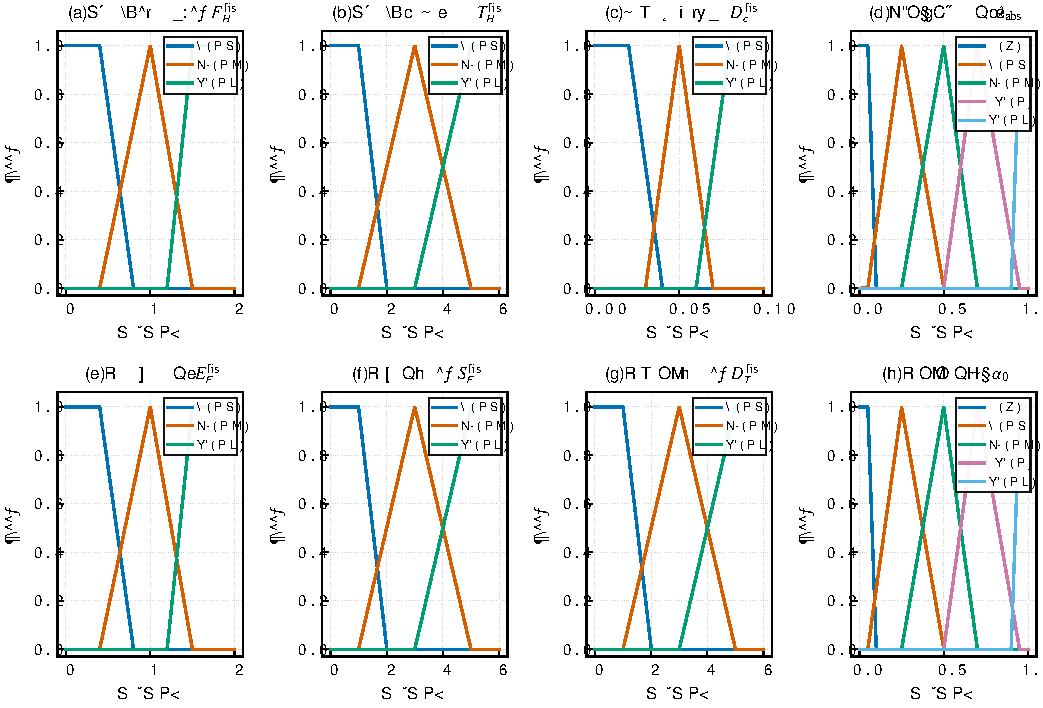
\includegraphics[width=0.98\textwidth]{figures/ch5/fuzzy_logic/ch5_fuzzy_membership_ieee.pdf}
  \caption{综合仲裁模糊逻辑控制器的输入与输出隶属函数}
  \label{fig:ch5_fuzzy_membership}
\end{figure}

图\ref{fig:ch5_fuzzy_membership}的上排对应参考层绝对通道。图\ref{fig:ch5_fuzzy_membership}(a)和图\ref{fig:ch5_fuzzy_membership}(b)分别描述操作者干预强度和持续时间的等级划分：短时弱输入主要落入“小”隶属区，持续增强的输入逐步激活“中”和“大”规则，从而避免把偶发抖动直接解释为明确的人类意图。图\ref{fig:ch5_fuzzy_membership}(c)给出了综合风险特征的隶属函数，其取值范围相对较窄，表示参考层对接触风险、方向分歧和几何裕度变化保持较高敏感度。图\ref{fig:ch5_fuzzy_membership}(d)为绝对通道输出，五个输出等级把人侧参考权重划分为从接近零到接近一的连续区间，使控制器既能保持自主参考主导，也能在操作者持续干预时平滑提高人侧安全参考的占比。

图\ref{fig:ch5_fuzzy_membership}的下排对应执行层力位仲裁。图\ref{fig:ch5_fuzzy_membership}(e)中的力误差输入越大，表示当前接触力越偏离期望区间；图\ref{fig:ch5_fuzzy_membership}(f)中的力安全裕度越大，表示接触力距离上下边界越远；图\ref{fig:ch5_fuzzy_membership}(g)中的切向位置裕度越大，表示轨迹误差越小、系统越有条件优先修正接触力。图\ref{fig:ch5_fuzzy_membership}(h)给出的 $\alpha_0$ 是执行层基础优先级，低等级对应更强的力调节倾向，高等级对应更强的位置和几何稳定倾向。由此，图\ref{fig:ch5_fuzzy_membership}不仅给出了模糊控制器的参数取值范围，也说明了后续调参时应当通过移动隶属函数中心、改变重叠宽度或调整输出等级中心来改变仲裁参数的响应速度和保守程度。

图\ref{fig:ch5_fuzzy_response}进一步展示两类模糊控制器的响应趋势。为便于二维显示，参考层绝对通道的综合风险特征固定为 $D_c^{\mathrm{fis}}=0.05$，参考层增量通道的风险变化率固定为 $\dot D_c^{\mathrm{fis}}=0$，执行层基础优先级响应中的力安全裕度固定为 $S_F^{\mathrm{fis}}=4.5$，方向修正响应中的基础优先级固定为 $\alpha_0=0.5$。这些固定量使每个响应面主要反映两个关键输入对输出的影响，而不改变前述模糊规则结构。

\begin{figure}[htbp]
  \centering
  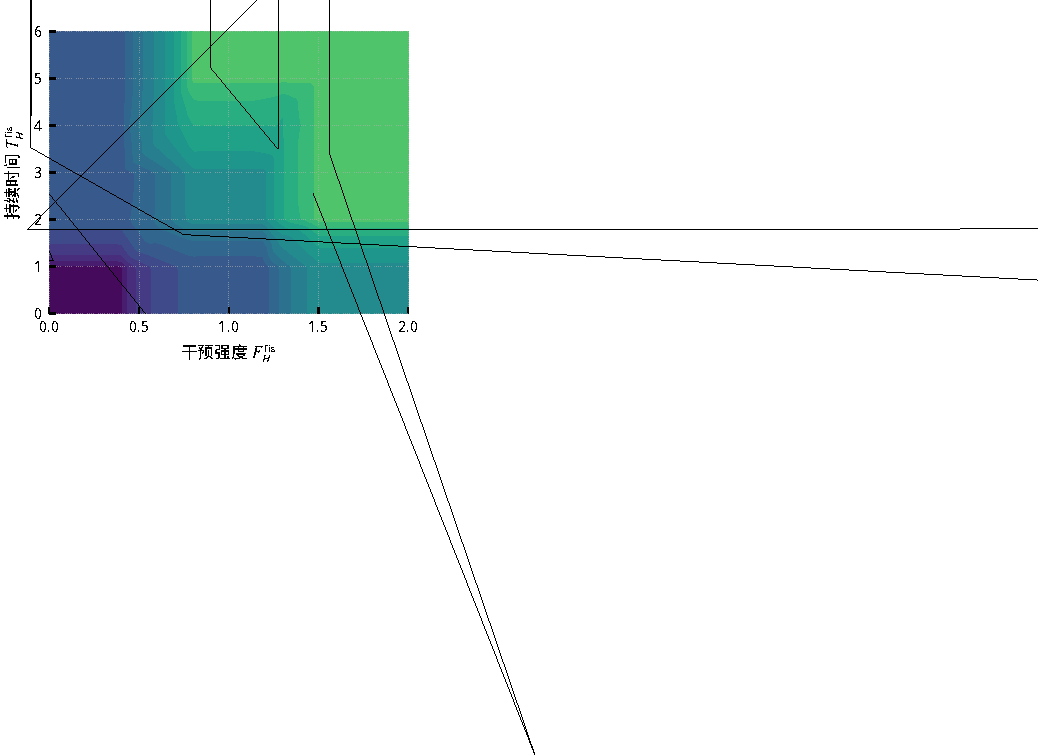
\includegraphics[width=0.92\textwidth]{figures/ch5/fuzzy_logic/ch5_fuzzy_response_ieee.pdf}
  \caption{综合仲裁模糊逻辑控制器的响应曲面}
  \label{fig:ch5_fuzzy_response}
\end{figure}

图\ref{fig:ch5_fuzzy_response}(a)表明，在风险特征保持中等时，$\lambda_{\mathrm{abs}}$ 随干预强度和持续时间共同增大而升高。当干预强度较小或持续时间较短时，输出保持在低权重区域，系统仍以自主参考为主；当两者同时进入中高等级时，输出向高权重区域过渡，说明操作者意图已经具备足够强度和持续性。图\ref{fig:ch5_fuzzy_response}(b)反映增量通道的作用：当干预强度变化率由负转正、持续时间趋势增强时，$\Delta\lambda_{\mathrm{inc}}$ 从负值区域过渡到正值区域，使参考层权重从回落转为上升；当输入趋势减弱时，增量通道提供负修正，促使系统逐步回到自主参考。

图\ref{fig:ch5_fuzzy_response}(c)展示执行层基础优先级 $\alpha_0$ 的变化规律。在切向位置裕度较大时，系统具有较好的轨迹状态，此时若力误差输入增大，模糊规则会降低 $\alpha_0$，把更多控制作用分配给接触力修正；在切向位置裕度较小时，即使存在力误差，输出也会保持较高优先级，以避免轨迹偏差继续扩大。图\ref{fig:ch5_fuzzy_response}(d)给出了边界方向修正的作用。横轴 $s_F<0$ 表示接触不足，控制器降低 $\alpha_{\mathrm{FP},r}$ 以增强接触恢复；横轴 $s_F>0$ 表示接触力接近上界，控制器提高 $\alpha_{\mathrm{FP},r}$ 以强化位置和几何稳定。纵轴 $\rho_F$ 越小，表示力安全裕度越低，方向修正项的幅值越大；$\rho_F$ 越接近 1，修正逐渐减弱，执行层更多依赖基础优先级 $\alpha_0$。因此，响应曲面从参数层面解释了双层仲裁在“人类意图增强、力误差增大、轨迹裕度下降、接触边界逼近”等典型状态下的连续切换规律。

表\ref{tab:ch5_fuzzy_parameter_effects}总结了主要参数对仲裁结果的影响。该表用于后续实验设置和敏感性分析，避免把模糊逻辑控制器理解为不可解释的经验规则。

\begin{table}[htbp]
  \centering
  \caption{模糊逻辑仲裁参数的作用趋势}
  \label{tab:ch5_fuzzy_parameter_effects}
  \small
  \begin{tabular}{@{}p{0.22\textwidth}p{0.34\textwidth}p{0.34\textwidth}@{}}
    \toprule
    参数或变量 & 增大时的物理含义 & 对仲裁参数的主要影响 \\
    \midrule
    $I_h$ 或 $F_H^{\mathrm{fis}}$ & 操作者输入更强 & $\lambda_{\mathrm{abs}}$ 增大，人侧安全参考更容易进入 $x_d$。 \\
    $T_h$ 或 $T_H^{\mathrm{fis}}$ & 输入持续时间更长 & 区分持续意图和短时扰动，持续输入使 $\alpha_{\mathrm{HR}}$ 上升更稳定。 \\
    $D_c$ 或 $D_c^{\mathrm{fis}}$ & 接触风险或方向分歧更明显 & 通过规则和安全投影共同限制危险法向输入，保留可行切向修正。 \\
    $\lambda_{\mathrm{HR}}$ & 参考层滤波响应更快 & $\alpha_{\mathrm{HR}}$ 更快靠近目标权重，但对手部抖动更敏感。 \\
    $E_F^{\mathrm{fis}}$ & 接触力误差更大 & 若位置裕度充足，$\alpha_0$ 降低并增强力调节；若位置误差已大，则保持位置恢复能力。 \\
    $S_F^{\mathrm{fis}}$ & 接触力安全裕度更大 & 允许规则更多依据力误差和位置裕度调节；裕度较低时方向修正作用增强。 \\
    $D_T^{\mathrm{fis}}$ & 切向位置误差更小 & 允许降低 $\alpha_0$ 修正力误差；该值降低时优先级升高以恢复轨迹。 \\
    $k_{\mathrm{up}}$ & 上界过压修正更强 & $s_F>0$ 且 $\rho_F$ 较低时更快提高 $\alpha_{\mathrm{FP},r}$。 \\
    $k_{\mathrm{low}}$ & 下界接触不足修正更强 & $s_F<0$ 且 $\rho_F$ 较低时更快降低 $\alpha_{\mathrm{FP},r}$。 \\
    $\lambda_{\mathrm{FP}}$ & 执行层优先级响应更快 & $\alpha_{\mathrm{FP}}$ 更快跟随接触状态变化，但过大时可能引入优先级抖动。 \\
    \bottomrule
  \end{tabular}
\end{table}

\subsection{组合方法与消融开关}
\label{subsec:ch5_method_switch_model}

为了让后续对比实验只改变指定模块，本章把完整组合方法写成统一开关模型。设 $\delta_H,\delta_P,\delta_F\in\{0,1\}$ 分别表示是否启用动态人机仲裁、安全参考投影和动态力位仲裁，固定人机权重和固定力位优先级分别为 $\bar\alpha_{\mathrm{HR}}$ 和 $\bar\alpha_{\mathrm{FP}}$。实验中的等效参考层权重、等效人侧参考、等效法向保留系数和等效执行层优先级为
\begin{equation}
  \begin{aligned}
  \alpha_{\mathrm{HR}}^{\delta}(t)
  &=
  \delta_H\alpha_{\mathrm{HR}}(t)
  +(1-\delta_H)\bar\alpha_{\mathrm{HR}},\\
  x_h^{\delta}(t)
  &=
  \delta_P x_h^{\mathrm{safe}}(t)
  +(1-\delta_P)x_h(t),\\
  \kappa_N^{\delta}(t)
  &=
  \delta_P\kappa_N(t)
  +(1-\delta_P),\\
  \alpha_{\mathrm{FP}}^{\delta}(t)
  &=
  \delta_F\alpha_{\mathrm{FP}}(t)
  +(1-\delta_F)\bar\alpha_{\mathrm{FP}}.
  \end{aligned}
  \label{eq:ch5_switch_variables}
\end{equation}
由此得到第 $i$ 组对比方法的期望轨迹和控制输入：
\begin{equation}
  \begin{aligned}
  x_d^{\delta}(t)
  &=
  x_r(t)+
  \alpha_{\mathrm{HR}}^{\delta}(t)P_T(t)
  \bigl(x_h^{\delta}(t)-x_r(t)\bigr)\\
  &\quad+
  \alpha_{\mathrm{HR}}^{\delta}(t)\kappa_N^{\delta}(t)P_N(t)
  \bigl(x_h^{\delta}(t)-x_r(t)\bigr),\\
  u^{\delta}(t)
  &=
  -K\bigl(\alpha_{\mathrm{FP}}^{\delta}(t),\hat K_e(t)\bigr)
  \xi^{\delta}(t).
  \end{aligned}
  \label{eq:ch5_switched_closed_loop}
\end{equation}
其中 $\xi^{\delta}$ 由 $x_d^{\delta}$ 和 $F_d$ 计算得到。固定参数基线取 $\delta_H=0,\delta_P=0,\delta_F=0$，仅参考层仲裁取 $\delta_H=1,\delta_P=1,\delta_F=0$，仅执行层调节取 $\delta_H=0,\delta_P=0,\delta_F=1$，完整组合方法取 $\delta_H=1,\delta_P=1,\delta_F=1$。若需要单独评估安全投影，可设置 $\delta_H=1,\delta_P=0,\delta_F=0$ 作为附加消融组。

对第 $i$ 组方法，统一记录的数据序列写为
\begin{equation}
  \mathcal D_i=
  \left\{
  x_k,x_{r,k},x_{h,k},x_{h,k}^{\mathrm{safe}},x_{d,k},
  y_{f,k},\rho_{F,k},\hat K_{e,k},
  \alpha_{\mathrm{HR},k},\alpha_{\mathrm{FP},k},
  u_k,e_{\mathrm{gc},k},T_{\mathrm{comp},k}
  \right\}_{k=1}^{N}.
  \label{eq:ch5_experiment_dataset}
\end{equation}
后续所有力安全、轨迹质量、人类修正和实时性指标均由 $\mathcal D_i$ 计算。这样处理可以把第五章的实验逻辑收束为三类问题：参考层是否正确处理人类输入，执行层是否正确处理力位折中，两层同时启用时是否在多指标上形成更稳定的综合表现。

\section{综合评价体系}
\label{sec:ch5_metrics}

综合评价体系由对比方法和评价指标两部分组成。对比方法用于回答每个模块是否必要，评价指标用于把模块作用落到可测量数据上。第五章主要验证既有控制器和仲裁器的组合效果，因此评价指标比理论推导更重要；所有指标应在结果图表前给出数学定义和物理解释。

对比方法分为固定参数基线、单层模块消融和完整组合方法三类。固定参数基线用于观察人工设定力位优先级在变刚度柔性接触中的局限，包含强位置优先、均衡优先和强力优先三组。强位置优先固定采用较高 $\alpha_{\mathrm{FP}}$，用于检验位置跟踪要求过强时的力安全风险；均衡优先固定采用中等 $\alpha_{\mathrm{FP}}$，作为常用人工折中基线；强力优先固定采用较低 $\alpha_{\mathrm{FP}}$，用于检验长期偏向力调节时可能产生的轨迹覆盖代价。三组固定方法均采用固定比例接受人类输入，因此不能根据人类输入类型和接触风险自动调整参考层权重。

单层模块消融用于分别考察第三章和第四章模块的贡献。仅参考层仲裁启用第四章动态人机仲裁和安全参考投影，但执行层保持中等固定力位优先级；若该方法能够提高安全切向修正接受率，却仍在高刚度区产生较长力越界时间，则说明参考层仲裁不能替代执行层动态力位调节。仅执行层调节启用第三章动态力位控制器，但固定或关闭人类修正；若该方法能够降低力越界时间，却无法跟随操作者安全切向修正，则说明执行层控制器不能单独完成在人监督下的任务覆盖调整。完整组合方法同时启用参考层动态仲裁、安全参考投影和执行层动态力位控制器，用于检验两层模块共同工作后的综合表现。仿真实验可保留上述六组方法以形成完整消融，实物实验可根据工作量选取均衡优先、仅参考层仲裁、仅执行层调节和完整组合方法四组，但中文代号和物理含义应保持一致。

力安全指标用于评价接触力调节精度和越界风险。设采样周期为 $T_s$，单次试验共有 $N$ 个采样点，受控法向接触力为 $y_{f,k}$，期望接触力为 $F_d$，接触力安全区间为 $[F_{\min},F_{\max}]$。接触力均方根误差定义为
\begin{equation}
  E_F^{\mathrm{RMS}}=
  \sqrt{\frac{1}{N}\sum_{k=1}^{N}\left(y_{f,k}-F_d\right)^2},
  \label{eq:ch5_metric_force_rms}
\end{equation}
力越界时间定义为
\begin{equation}
  T_{\mathrm{vio}}=
  T_s\sum_{k=1}^{N}\mathbb I\left(y_{f,k}<F_{\min}\ \mathrm{or}\ y_{f,k}>F_{\max}\right).
  \label{eq:ch5_metric_violation_time}
\end{equation}
其中 $E_F^{\mathrm{RMS}}$ 描述接触力跟踪期望值的平均偏差，$T_{\mathrm{vio}}$ 描述接触力离开安全区间的累计时间。二者共同反映接触稳定性和安全性，后者对高刚度区域或危险法向输入更敏感。

轨迹质量指标用于评价机器人是否完成期望接触路径。设实际接触点位置为 $x_k$，最终期望轨迹为 $x_{d,k}$，则轨迹均方根误差定义为
\begin{equation}
  E_x^{\mathrm{RMS}}=
  \sqrt{\frac{1}{N}\sum_{k=1}^{N}\left\|x_k-x_{d,k}\right\|^2}.
  \label{eq:ch5_metric_position_rms}
\end{equation}
若需要评价运动平滑性，可使用任务空间 jerk 指标
\begin{equation}
  J_x=
  \sqrt{\frac{1}{N}\sum_{k=1}^{N}\left\|\dddot x_k\right\|^2}.
  \label{eq:ch5_metric_jerk}
\end{equation}
实物实验中三阶差分容易放大测量噪声，计算 $J_x$ 时应使用统一滤波后的轨迹数据，并在结果分析中说明滤波窗口。轨迹指标不单独代表任务优劣，需要与力安全指标和人类修正指标共同解释。

人机协同指标用于评价操作者输入是否以合理方式影响最终期望轨迹。设 $\mathcal K_T$ 为安全切向修正时间段，$\mathcal K_N$ 为危险法向输入时间段，$x_{r,k}$ 为自主参考，$x_{h,k}$ 为人侧候选参考，$x_{d,k}$ 为最终期望轨迹。人类修正接受率定义为
\begin{equation}
  R_{\mathrm{acc}}=
  \frac{\sum_{k\in\mathcal K_T}\left\|x_{d,k}-x_{r,k}\right\|}
  {\sum_{k\in\mathcal K_T}\left\|x_{h,k}-x_{r,k}\right\|+\varepsilon},
  \label{eq:ch5_metric_acceptance}
\end{equation}
其中 $\varepsilon>0$ 用于避免分母为零。$R_{\mathrm{acc}}$ 越大，说明安全切向修正越多地进入最终期望轨迹。设 $d_{h,k}^{N}$ 和 $d_{d,k}^{N}$ 分别为人侧候选参考和最终期望轨迹中的法向压入量，则危险输入抑制率定义为
\begin{equation}
  R_{\mathrm{sup}}=
  1-
  \frac{\sum_{k\in\mathcal K_N}\max\{d_{d,k}^{N},0\}}
  {\sum_{k\in\mathcal K_N}\max\{d_{h,k}^{N},0\}+\varepsilon}.
  \label{eq:ch5_metric_suppression}
\end{equation}
该指标只在预先设置的危险法向输入时间段内计算。$R_{\mathrm{sup}}$ 越大，说明参考层安全投影和动态仲裁对危险输入的削弱越充分。

带远心运动约束的长工具实验还需要几何误差指标。设第 $k$ 个采样点的固定点轴线误差为 $e_{\mathrm{gc},k}$，则
\begin{equation}
  E_{\mathrm{gc}}^{\mathrm{RMS}}=
  \sqrt{\frac{1}{N}\sum_{k=1}^{N}e_{\mathrm{gc},k}^{2}},
  \qquad
  E_{\mathrm{gc}}^{\max}=\max_{k}e_{\mathrm{gc},k}.
  \label{eq:ch5_metric_gc}
\end{equation}
其中 $E_{\mathrm{gc}}^{\mathrm{RMS}}$ 反映整个任务过程中的平均几何偏离，$E_{\mathrm{gc}}^{\max}$ 反映最不利时刻的固定点轴线误差。该指标用于长工具任务的边界条件评价，不作为无远心运动约束表面操作实验的核心指标。

综合评分用于辅助比较同一工况下的多指标表现。设 $\tilde E_F$、$\tilde T_{\mathrm{vio}}$、$\tilde E_x$、$\tilde T_{\mathrm{comp}}$ 和 $\tilde E_{\mathrm{gc}}$ 为归一化后的指标，$T_{\mathrm{comp}}$ 为单周期计算时间，则可定义
\begin{equation}
  S=
  w_F\tilde E_F+
  w_V\tilde T_{\mathrm{vio}}+
  w_X\tilde E_x+
  w_A(1-R_{\mathrm{acc}})+
  w_S(1-R_{\mathrm{sup}})+
  w_C\tilde T_{\mathrm{comp}}+
  w_G\tilde E_{\mathrm{gc}}.
  \label{eq:ch5_metric_score}
\end{equation}
其中 $w_F,w_V,w_X,w_A,w_S,w_C,w_G$ 为非负权重，并在实验前固定。无远心运动约束任务可令 $w_G=0$。综合评分只用于同一任务和同一归一化规则下的方法比较，正式分析仍应回到各单项指标，说明不同方法在力安全、轨迹质量、人类修正和实时性之间的折中关系。

\section{综合仿真验证}
\label{sec:ch5_integrated_simulation}

综合仿真用于在可重复条件下完成完整消融和参数预筛选。与第三章只考察执行层力位控制器、第四章只考察参考层人机仲裁器不同，本节把两类模块同时接入同一闭环，使每组方法面对完全相同的自主轨迹、人类输入序列、柔性环境参数和接触力边界。这样处理可以把方法差异限制在参考层仲裁和执行层力位调节本身，避免由任务轨迹、材料参数或输入时刻不同造成比较偏差。

\subsection{仿真工况设置}
\label{subsec:ch5_simulation_task_setting}

仿真任务采用柔性表面扫描模型。机器人末端工具沿表面切向完成一条名义扫描路径，法向保持期望接触力，柔性材料由低刚度区、高刚度区、局部缺陷区和名义刚度失配区组成。低刚度区用于模拟泡棉、软硅胶或柔性密封件，接触力容易低于有效接触下界；高刚度区用于模拟局部支撑增强、材料加厚或曲面边缘，按照名义深度推进时容易产生过压；局部缺陷区不作为不可穿越障碍，而作为操作者希望绕行或额外覆盖的工艺区域。该设置使同一条扫描任务同时包含环境刚度变化、人类切向修正和危险法向输入，能够检验两层模块是否在多因素耦合下保持可解释响应。

仿真控制周期取 $T_s=0.01\,\mathrm{s}$，单次扫描时间取 $48\,\mathrm{s}$，切向扫描范围为 $0\sim0.12\,\mathrm{m}$。接触力安全下界、期望值和上界分别设为 $F_{\min}=0.38\,\mathrm{N}$、$F_d=0.70\,\mathrm{N}$ 和 $F_{\max}=1.16\,\mathrm{N}$。名义扫描深度按 $K_{\mathrm{nom}}=520\,\mathrm{N/m}$ 生成，而实际分段刚度取 $320\,\mathrm{N/m}$、$860\,\mathrm{N/m}$、$230\,\mathrm{N/m}$ 和 $1120\,\mathrm{N/m}$。名义刚度与实际刚度不一致是仿真工况的关键：如果控制器只依赖固定参数，低刚度段容易接触不足，高刚度段容易力越界；若动态力位优先级有效，则应在接触力裕度降低和估计刚度升高时自动改变执行折中。

人类输入序列由三类片段组成。安全切向修正片段中，操作者沿表面切向给出持续位移，用于绕开缺陷区域或改变扫描带宽；参考层应提高 $\alpha_{\mathrm{HR}}$，使该修正进入 $x_d$。危险法向压入片段中，操作者沿接触法向继续压入柔性材料；参考层安全投影应削弱该法向分量，执行层应根据 $\rho_F$ 和 $s_F$ 调整 $\alpha_{\mathrm{FP}}$，避免接触力越过上界。短时扰动片段中，输入持续时间较短且方向不稳定；仲裁权重不应发生明显突跳，最终期望轨迹应保持平滑。上述输入片段的时间窗在所有方法中保持一致，从而使人类修正接受率和危险输入抑制率具有可比性。

\subsection{仿真对比设置}
\label{subsec:ch5_simulation_method_setting}

综合仿真保留六组对比方法。强位置优先、均衡优先和强力优先分别固定执行层力位优先级，用于观察固定折中点在不同刚度段的失配现象。强位置优先能够较好保持名义轨迹，但高刚度段更容易出现力峰值；强力优先通常能降低接触力均方根误差，却可能牺牲轨迹覆盖和人类切向修正效果；均衡优先提供人工折中参考。仅参考层仲裁启用第四章动态人机仲裁与安全投影，但执行层保持固定中等力位优先级，用于判断参考层是否足以处理全部接触风险。仅执行层调节启用第三章动态力位控制器，但不接受人类修正，用于判断执行层能否在缺少人类监督时完成任务覆盖调整。完整组合方法同时启用 $\alpha_{\mathrm{HR}}$、安全投影和 $\alpha_{\mathrm{FP}}$，是本章需要验证的集成方案。

仿真数据按统一时间窗计算。接触建立前的过渡阶段不纳入正式统计，接触力进入安全区间并稳定保持后开始评价。每组方法记录 $x_r$、$x_h$、$x_h^{\mathrm{safe}}$、$x_d$、实际末端位置、接触力、估计刚度、$\rho_F$、$\alpha_{\mathrm{HR}}$、$\alpha_{\mathrm{FP}}$、控制输入和单周期计算时间。对同一组数据同时计算力安全指标、轨迹质量指标、人类修正指标和综合评分。综合评分的归一化基准在所有方法计算前固定，避免事后调权改变排序。

已有综合仿真结果可作为后续实物实验参数选择的依据。在该工况下，强位置优先的接触力越界时间达到 $20.10\,\mathrm{s}$，说明固定高位置优先级在高刚度区具有明显过压风险；强力优先的力均方根误差为 $0.204\,\mathrm{N}$，略低于完整组合方法，但其安全切向修正接受率保持在 $0.58$，危险输入抑制率也只有 $0.42$。仅参考层仲裁能够把接受率提高到 $0.89$，危险输入抑制率提高到 $0.91$，但由于执行层仍为固定优先级，力越界时间仍为 $4.50\,\mathrm{s}$。仅执行层调节的力越界时间下降到 $1.52\,\mathrm{s}$，但因不接受人类修正，轨迹误差上升到 $5.63\,\mathrm{mm}$。完整组合方法的综合评分为 $3.843$，低于最佳固定参数方法的 $4.735$，同时保持 $0.89$ 的切向修正接受率和 $0.93$ 的危险输入抑制率。该结果说明完整组合方法的优势不在于所有单项指标均最小，而在于力安全、轨迹质量和人类修正之间形成了更均衡的折中。

\subsection{仿真结果分析口径}
\label{subsec:ch5_simulation_analysis_setting}

仿真结果分析按总体统计、典型时序和局部片段三个层次展开。总体统计用于比较六组方法的综合评分、接触力均方根误差、力越界时间、轨迹误差、人类修正接受率和危险输入抑制率。典型时序用于解释 $\alpha_{\mathrm{FP}}$ 是否随估计刚度和力安全裕度变化：当 $\hat K_e$ 升高且 $\rho_F$ 降低时，完整组合方法应降低位置优先级以释放力调节能力；当接触力回到安全区间中部时，$\alpha_{\mathrm{FP}}$ 应逐步恢复，使机器人继续推进扫描轨迹。局部片段用于解释参考层动态仲裁：安全切向修正片段应观察 $x_d$ 是否偏向 $x_h^{\mathrm{safe}}$，危险法向输入片段应观察 $x_h$ 与 $x_h^{\mathrm{safe}}$ 的法向差异以及接触力峰值是否被抑制。

若某个基线在单项指标上表现较好，分析中应保留该现象。例如强力优先在当前仿真中得到较小力均方根误差，这是长期偏向力调节的直接结果；但它不能根据人类输入类型调整参考层权重，因此难以同时保证安全切向修正保留和危险法向输入抑制。仅执行层调节可以降低越界时间，却把任务退化为无人类监督的自动扫描。仅参考层仲裁可以保留人的轨迹经验，但在高刚度段仍受固定执行层优先级限制。完整组合方法的结论应表述为在所设柔性表面扫描工况下具有更好的综合表现，而不是在所有指标上全面优于所有方法。

\section{表面操作实验}
\label{sec:ch5_surface_experiment}

表面操作实验用于验证完整组合方法在无远心运动约束的普通柔性接触任务中的可执行性。该实验不依赖长工具或套管结构，主要面向柔性材料扫描、接触式检测、软质工件表面处理等一般任务。设置该实验的目的，是避免第五章只在长工具或手术训练边界下成立，使读者能够看到第三章执行层控制器和第四章参考层仲裁器在普通柔性物体操作中的共同作用。

\subsection{平台与材料设置}
\label{subsec:ch5_surface_platform}

实验平台采用 Franka 机械臂或等效七自由度机械臂，末端安装圆头探针或短杆接触工具。工具端部应保持圆滑，避免尖锐边缘破坏柔性材料。柔性对象可选海绵、硅胶块、泡棉或软质橡胶条，材料固定在刚性平板上。为形成可重复的变刚度区域，可将两种不同硬度材料沿扫描方向拼接，也可在同一软垫下方局部增加硬质支撑。实验前通过低速压入或小幅扫描估计各区域的表观刚度范围，并据此设置期望接触力和安全边界。若采用典型软垫材料，接触力可取 $F_d=0.7\,\mathrm{N}$ 左右，安全区间可按材料耐受能力设置为 $[0.3,1.2]\,\mathrm{N}$ 附近；正式实验中应以材料不产生明显永久变形为硬约束。

操作者输入由主端设备、手柄或预设输入序列给出。为保证不同方法可比，主要重复试次采用相同预设输入序列；在完成可重复数据后，可补充少量真实操作者试次用于展示人机交互可行性。输入序列包含两个核心时间段：其一为切向安全修正，操作者沿表面横向移动参考轨迹，使机器人绕开标记区域或增加扫描覆盖；其二为法向危险压入，操作者沿接触法向给出短时或持续压入，用于检验安全投影和执行层力位调节。机器人自主参考路径可设置为直线扫描或轻微曲线扫描，路径长度控制在 $8\sim12\,\mathrm{cm}$，单次实验时长控制在 $30\sim60\,\mathrm{s}$，以保证操作者输入、刚度变化和接触建立阶段均能被清楚记录。

\subsection{实验流程与对比方法}
\label{subsec:ch5_surface_protocol}

每次表面操作实验开始前，机器人先进入安全初始位姿，末端工具在柔性材料上方保持小间隙。力传感器或外力估计通道静止采样数秒，用于计算零偏。随后机器人以低速接近材料，接触力进入安全区间后开始正式记录。正式任务阶段，机器人沿名义路径扫描，操作者输入在预设时间窗内生效。任务结束后，机器人沿法向缓慢卸载并退出工作区。若实验过程中触发硬力阈值、速度上限或急停，试次单独标记为工程异常，不与正常试次混合统计。

表面操作实验建议至少比较四组方法：均衡优先、仅参考层仲裁、仅执行层调节和完整组合方法。均衡优先提供常用固定参数基线；仅参考层仲裁用于观察安全切向修正是否能够进入轨迹，但高刚度区力越界是否仍较明显；仅执行层调节用于观察动态力位控制能否降低力越界，但是否牺牲人类修正；完整组合方法用于观察两类模块是否同时发挥作用。若实验时间允许，可增加强位置优先和强力优先两组，用于补充固定优先级的上下界表现。每组方法建议重复三次，条件允许时重复五次。对重复试次计算均值和标准差，典型时序曲线选择接触稳定、输入执行完整且无硬安全中断的一次试次展示。

表面操作实验的主要记录量包括接触力、期望接触力、机器人实际轨迹、自主参考、人侧候选参考、安全人侧参考、最终期望轨迹、$\alpha_{\mathrm{HR}}$、$\alpha_{\mathrm{FP}}$、力安全裕度、估计刚度、控制输入和单周期计算时间。结果分析中，切向修正阶段重点计算 $R_{\mathrm{acc}}$ 和切向轨迹偏移误差；危险法向输入阶段重点计算 $R_{\mathrm{sup}}$、接触力峰值和力越界时间；全任务范围内计算接触力均方根误差、轨迹均方根误差和控制周期统计。若完整组合方法在力均方根误差上略高于强力优先或仅执行层调节，应结合人类修正接受率和轨迹覆盖说明其综合折中，而不应把单项力误差解释为唯一目标。

\section{长工具操作实验}
\label{sec:ch5_long_tool_experiment}

长工具操作实验用于验证完整组合方法在固定点轴线边界下的可执行性。该实验对应机器人辅助手术训练、狭窄入口操作和长工具柔性接触等场景，但在本章中只作为一类几何边界条件出现。实验重点不是提出新的远心运动控制器，而是在长工具通过固定孔或套管接触柔性材料时，检验参考层人机仲裁和执行层力位调节是否仍能协同工作。

\subsection{长工具平台与几何标定}
\label{subsec:ch5_long_tool_platform}

实验平台采用机械臂末端安装长杆、腹腔镜等效工具或其他细长接触工具。工具通过固定孔、套管或刚性夹具形成远心运动边界，柔性对象布置在固定孔下方或工具远端可达区域内。固定点位置记为 $p_r$，工具轴线上一点记为 $p_t$，工具轴线单位方向记为 $a_t$，固定点到工具轴线的几何误差定义为
\begin{equation}
  e_{\mathrm{gc}}=
  \left\|
  \left(I-a_ta_t^{\mathrm T}\right)(p_r-p_t)
  \right\|.
  \label{eq:ch5_gc_distance_experiment}
\end{equation}
若固定点位于工具轴线上，则 $e_{\mathrm{gc}}=0$；误差越大，说明工具轴线偏离固定孔或套管中心越明显。该误差由工具几何和法兰位姿计算得到，不需要额外视觉系统。实验前应标定法兰到工具接触点的长度、工具轴线方向、固定孔中心位置以及接触点与柔性材料的初始相对位置。若套管间隙或工具柔顺性造成几何误差下限，应在实验设置中记录该工程边界。

长工具任务不宜设置过长路径或复杂三维轨迹。建议采用 $3\sim5\,\mathrm{cm}$ 的短距离扫描或点到点接触任务，单次时长控制在 $30\sim60\,\mathrm{s}$。期望接触力应低于表面操作实验，可根据工具端部和柔性材料安全范围设置在 $0.3\sim0.6\,\mathrm{N}$。操作者输入同样包括切向修正和法向误推两类：切向修正用于改变工具端部在柔性材料上的扫描带，法向误推用于检验安全投影和执行层调节能否降低过压风险。由于长工具通过固定点运动，参考层生成的 $x_d$ 还需经过工具几何映射和速度限幅，保证工具轴线不会因人类输入突变而明显偏离固定点。

\subsection{长工具实验流程}
\label{subsec:ch5_long_tool_protocol}

实验开始前，先确认固定孔、工具和柔性材料的相对位置，使工具在无接触状态下通过固定点附近并保持足够间隙。随后机器人缓慢接近柔性材料，形成稳定轻触接触后进入正式扫描。每次试验记录工具轴线、接触点位置、法兰位姿、受控法向力、最终期望轨迹、两类仲裁参数和固定点轴线误差。若工具与套管发生明显碰撞、固定结构松动或接触力触发硬阈值，该试次不作为正常性能统计，而应作为安全事件单独说明。

长工具实验建议至少包含均衡优先、仅执行层调节和完整组合方法三组。若平台稳定且实验时间允许，可增加仅参考层仲裁，以更完整地分离参考层和执行层作用。均衡优先用于观察固定参数在长工具场景下的基准表现；仅执行层调节用于观察力位控制器在固定参考下能否降低力越界和几何误差；完整组合方法用于验证操作者安全切向修正能否进入工具端轨迹，同时危险法向压入是否被削弱。每组方法建议重复三次，若工具装夹和材料回复性较好，可重复五次。为降低被试差异，主要对比仍采用预设输入序列；真实操作者输入可作为补充展示。

结果分析需要同时观察接触力和几何误差。若完整组合方法降低了危险法向输入阶段的接触力峰值，但 $E_{\mathrm{gc}}^{\mathrm{RMS}}$ 或 $E_{\mathrm{gc}}^{\max}$ 明显增大，则说明参考层修正或速度限幅仍需调整；若几何误差保持在基线相近水平，同时力越界时间下降、切向修正接受率提高，则说明两层模块在长工具边界下具有可执行性。考虑到套管间隙、工具柔顺性和标定误差会影响几何指标，结论应写为完整组合方法未明显恶化固定点轴线误差，而不是声称实现高精度远心运动控制。

\section{参数敏感性与结构消融}
\label{sec:ch5_sensitivity_ablation}

参数敏感性用于说明第五章实验参数不是任意选取的经验值，而是受到接触力安全、轨迹平滑性和人机交互响应共同约束。大规模参数网格主要在仿真中完成，实物实验只选择少量关键参数做验证。这样既能覆盖参数变化趋势，又不会显著增加实物平台风险。

\subsection{敏感性参数设置}
\label{subsec:ch5_sensitivity_setting}

敏感性分析选择四类参数。第一类是执行层优先级下限 $\alpha_{\min}$。若下限过高，控制器在接触力接近边界时仍保持较强位置跟踪，容易增加力峰值和越界时间；若下限过低，系统可能过度偏向力调节，造成切向推进滞后和轨迹覆盖下降。第二类是执行层滤波速度 $\lambda_{\mathrm{FP}}$。取值过小会使力位优先级响应滞后，进入高刚度区后卸载不及时；取值过大则可能放大力传感器噪声，引入力位优先级抖动。第三类是参考层滤波速度 $\lambda_{\mathrm{HR}}$。取值过小会使操作者持续修正难以及时进入轨迹；取值过大则可能把手部抖动或短时误触放大为期望轨迹突变。第四类是力安全余量 $\Delta_F$。余量过小会削弱危险输入抑制效果，余量过大则使系统过于保守，安全切向修正也可能被过度削弱。

每类参数可采用慢、中、快三档或小、中、大三档设置。仿真中每档使用相同扫描路径、相同人类输入序列和相同分段刚度环境，并计算 $T_{\mathrm{vio}}$、$E_x^{\mathrm{RMS}}$、$R_{\mathrm{acc}}$、$R_{\mathrm{sup}}$、$\operatorname{RMS}(\dot\alpha_{\mathrm{FP}})$ 和 $\operatorname{RMS}(\dot\alpha_{\mathrm{HR}})$。实物实验可只选择 $\lambda_{\mathrm{FP}}$ 和 $\Delta_F$ 两类参数，每档重复三次。敏感性分析的目标不是寻找全局最优参数，而是确认参数变化方向与方法机理一致，并为正式实验选择中档参数提供依据。

\subsection{结构消融设置}
\label{subsec:ch5_ablation_setting}

结构消融围绕三类模块展开。关闭安全投影时，系统仍可根据人类输入生成动态 $\alpha_{\mathrm{HR}}$，但人侧候选参考不再投影到安全集合；该组用于检验危险法向输入是否会直接推高接触力。固定执行层优先级时，参考层动态仲裁仍然存在，但 $\alpha_{\mathrm{FP}}$ 保持中等常值；该组用于检验变刚度区和低力安全裕度下是否需要执行层动态调节。固定人机权重时，执行层力位控制器仍然启用，但参考层不能根据输入强度、持续时间和风险状态调整人类影响程度；该组用于检验操作者安全切向修正是否会被不足接受，短时扰动是否更容易进入轨迹。完整组合方法作为对照，同时保留安全投影、动态人机仲裁和动态力位调节。

消融结果应与第三章、第四章的作用边界对应解释。若关闭安全投影后危险法向输入阶段的接触力峰值上升，说明第四章安全参考生成在第五章综合任务中不可替代。若固定执行层优先级后高刚度区越界时间增加，说明第三章动态力位控制器在组合闭环中仍然发挥作用。若固定人机权重后切向修正接受率下降或短时扰动影响变大，说明参考层动态仲裁不仅是形式上的共享控制权重，而是影响最终期望轨迹质量的必要模块。若完整组合方法在综合评分上优于各消融组，但在某个单项指标上不是最优，分析仍应回到力安全、轨迹质量、人类修正和实时性的整体折中。

\section{本章小结}
\label{sec:ch5_summary}

本章围绕人机协同柔性物体操作，对第三章执行层力位协同控制器和第四章参考层动态仲裁方法进行了统一建模和综合实验设置。首先明确了综合验证目标，说明本章关注的是两类模块在同一闭环中的兼容性、可执行性和跨边界条件适用性，而不是提出新的独立控制理论。随后给出了统一实验系统、信号流、数据记录规范和评价指标，使无远心运动约束表面操作、带远心运动约束长工具操作以及仿真敏感性分析可以使用相同符号和指标体系进行比较。

在方法建模上，本章将 $\alpha_{\mathrm{HR}}$ 限定为参考层人机仲裁权重，将 $\alpha_{\mathrm{FP}}$ 限定为执行层力位优先级。参考层通过人侧安全参考、切向和法向分解以及动态滤波保留安全修正并削弱危险输入；执行层根据接触力安全裕度、力误差和切向位置裕度调节力位反馈优先级。模糊逻辑仲裁参数设计进一步说明了两类权重的输入、输出、规则激活和参数影响趋势，使后续实验中的权重变化具有可解释性。

在实验安排上，本章设置综合仿真、表面操作实验、长工具操作实验以及参数敏感性和结构消融。综合仿真用于完成六组方法的完整消融和参数预筛选；表面操作实验用于验证方法在一般柔性表面接触任务中的实物可执行性；长工具操作实验用于检验方法在固定点轴线边界下是否仍能保持力安全和几何约束；敏感性与消融分析用于解释参数选择和模块必要性。后续结果分析应坚持有边界的结论表述：完整组合方法的目标是在所设工况下取得力安全、轨迹质量、人类修正和实时性之间的综合折中，而不是在所有单项指标上都取得最小误差。
